\testfile{pgfplotstest.reverseaxis.tex}
{
	\pgfplotsset{compat=newest}
	\def\showit#1#2{%
		\node[pin=#2:(s.#1),fill=black,circle,scale=0.3] at (current axis.#1) {};
	}%
	\tikzstyle{every pin}=[opacity=0.5,fill=yellow,rectangle,rounded corners=3pt,font=\tiny]
	\def\showallanchors{
		\showit{north}{90}
		\showit{north west}{135}
		\showit{west}{180}
		\showit{south west}{225}
		\showit{south}{270}
		\showit{south east}{305}
		\showit{east}{0}
		\showit{north east}{45}
		\showit{center}{90}
		{\pgfplotsset{every pin/.append style={pin distance=1cm}}%
		\showit{above origin}{45}
		}%
		\showit{right of origin}{45}
		{\pgfplotsset{every pin/.append style={pin distance=1cm}}%
		\showit{below origin}{0}
		}%
		\showit{left of origin}{135}
		\showit{origin}{135}
	}
	\let\showanchorsafteraxis=\showallanchors
	%\pgfplotsset{extra description/.append code={\showallanchors}}
	\let\showanchorsafteraxis=\relax

	\testsection{x dir=reverse}
	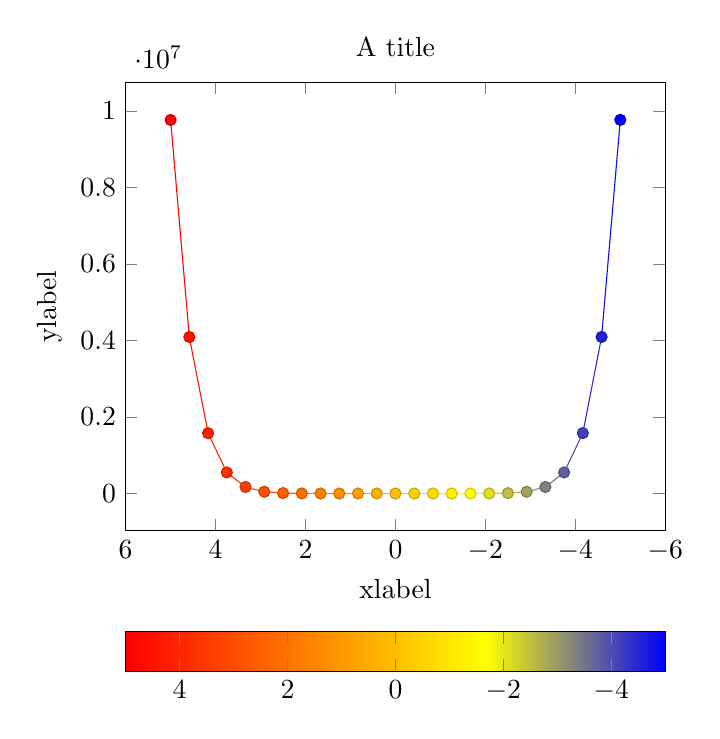
\begin{tikzpicture}
		\begin{axis}[
			x dir=reverse,
			title=A title,
			xlabel=xlabel,
			ylabel=ylabel,
			colorbar horizontal,
			colorbar style={x dir=reverse},
		]
		\addplot+[mesh,scatter,scatter src=x] {x^10};
		\end{axis}
		\showanchorsafteraxis
	\end{tikzpicture}

	\testsection{x dir=reverse,axis lines=left}
	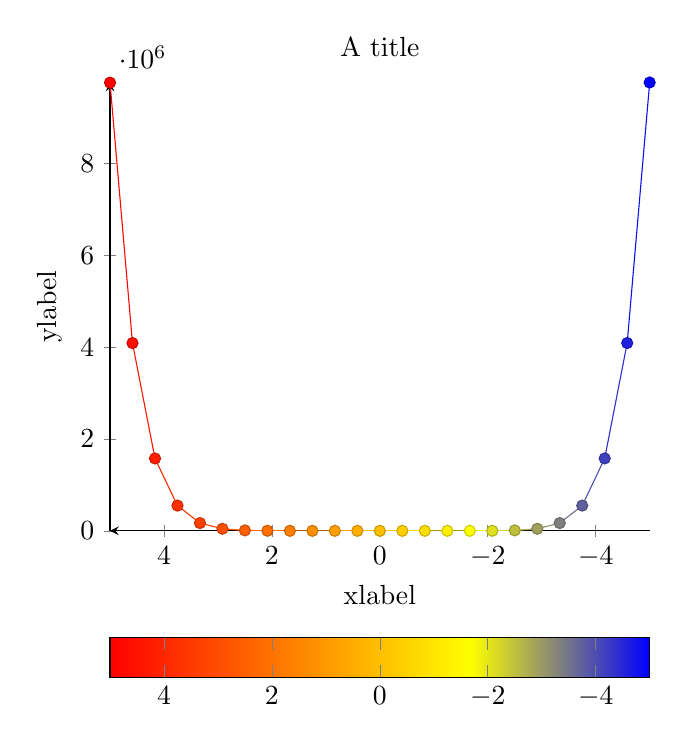
\begin{tikzpicture}
		\begin{axis}[
			axis lines=left,
			x dir=reverse,
			title=A title,
			xlabel=xlabel,
			ylabel=ylabel,
			colorbar horizontal,
			colorbar style={x dir=reverse},
		]
		\addplot+[mesh,scatter,scatter src=x] {x^10};
		\end{axis}
		\showanchorsafteraxis
	\end{tikzpicture}
	
	\testsection{x dir=reverse,axis lines=center}
	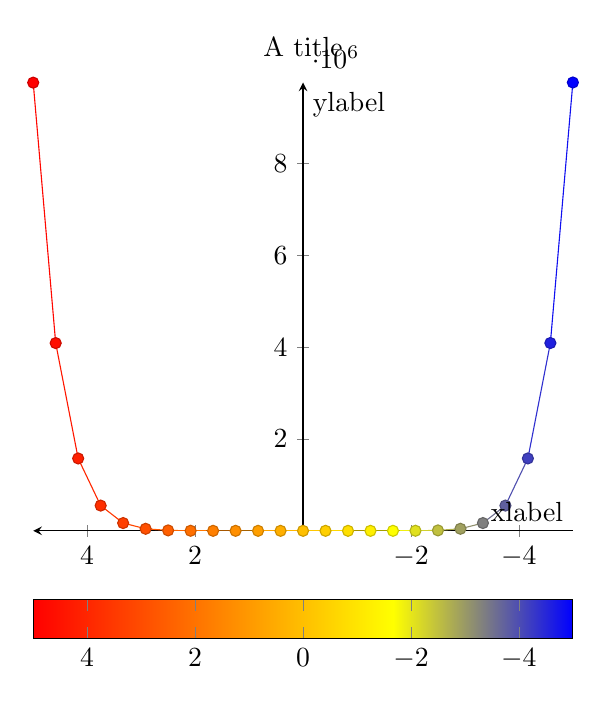
\begin{tikzpicture}
		\begin{axis}[
			axis lines=center,
			x dir=reverse,
			title=A title,
			xlabel=xlabel,
			ylabel=ylabel,
			colorbar horizontal,
			colorbar style={x dir=reverse},
		]
		\addplot+[mesh,scatter,scatter src=x] {x^10};
		\end{axis}
		\showanchorsafteraxis
	\end{tikzpicture}

	\testsection{x dir=reverse,axis lines=right}
	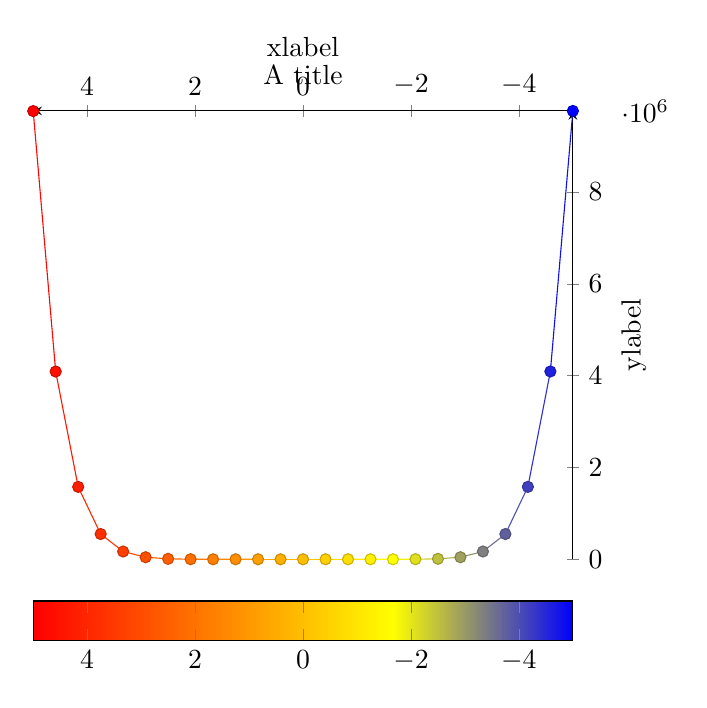
\begin{tikzpicture}
		\begin{axis}[
			axis lines=right,
			x dir=reverse,
			title=A title,
			xlabel=xlabel,
			ylabel=ylabel,
			colorbar horizontal,
			colorbar style={x dir=reverse},
		]
		\addplot+[mesh,scatter,scatter src=x] {x^10};
		\end{axis}
		\showanchorsafteraxis
	\end{tikzpicture}

	\testsection{y dir=reverse}
	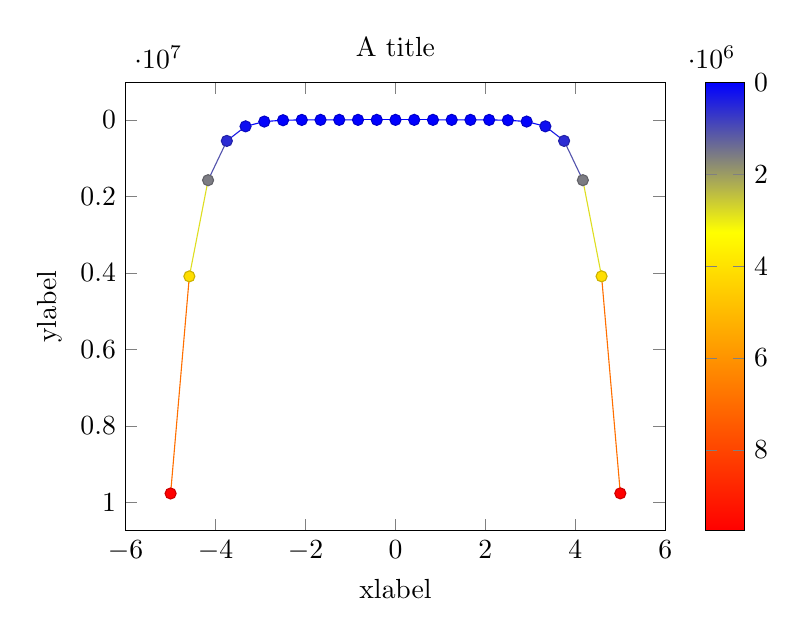
\begin{tikzpicture}
		\begin{axis}[
			y dir=reverse,
			title=A title,
			xlabel=xlabel,
			ylabel=ylabel,
			colorbar,
			clip=false,
			colorbar style={y dir=reverse,clip=false},
		]
		\addplot+[mesh,scatter] {x^10};
		\end{axis}
		\showanchorsafteraxis
	\end{tikzpicture}

	\testsection{y dir=reverse,axis lines=left}
	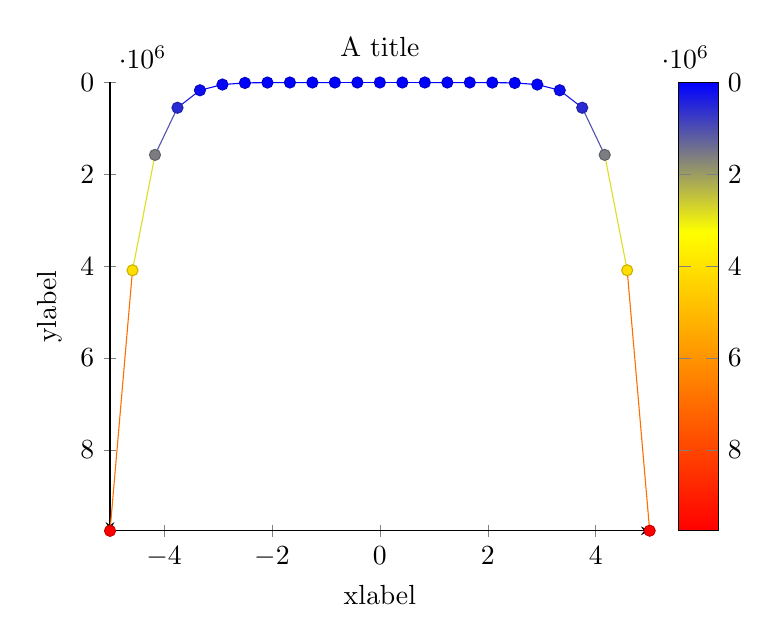
\begin{tikzpicture}
		\begin{axis}[
			axis lines=left,
			y dir=reverse,
			title=A title,
			xlabel=xlabel,
			ylabel=ylabel,
			colorbar,
			colorbar style={y dir=reverse},
		]
		\addplot+[mesh,scatter] {x^10};
		\end{axis}
		\showanchorsafteraxis
	\end{tikzpicture}
	
	\testsection{y dir=reverse,axis lines=center}
	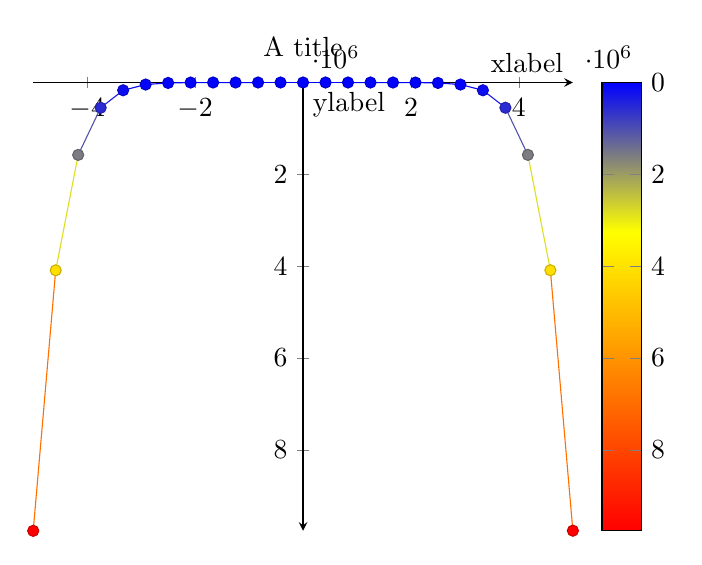
\begin{tikzpicture}
		\begin{axis}[
			axis lines=center,
			y dir=reverse,
			title=A title,
			xlabel=xlabel,
			ylabel=ylabel,
			colorbar,
			colorbar style={y dir=reverse},
		]
		\addplot+[mesh,scatter] {x^10};
		\end{axis}
		\showanchorsafteraxis
	\end{tikzpicture}

	\testsection{y dir=reverse,axis lines=right}
	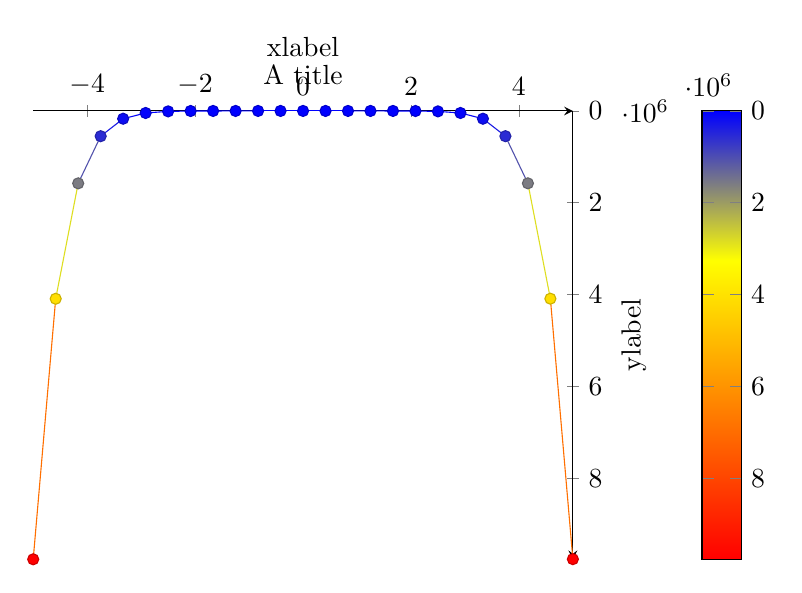
\begin{tikzpicture}
		\begin{axis}[
			axis lines=right,
			y dir=reverse,
			title=A title,
			xlabel=xlabel,
			ylabel=ylabel,
			colorbar,
			colorbar style={y dir=reverse},
		]
		\addplot+[mesh,scatter] {x^10};
		\end{axis}
		\showanchorsafteraxis
	\end{tikzpicture}
}
